
\subsection{Polarized target}\label{poltar-section}
\begin{figure}
\begin{center}
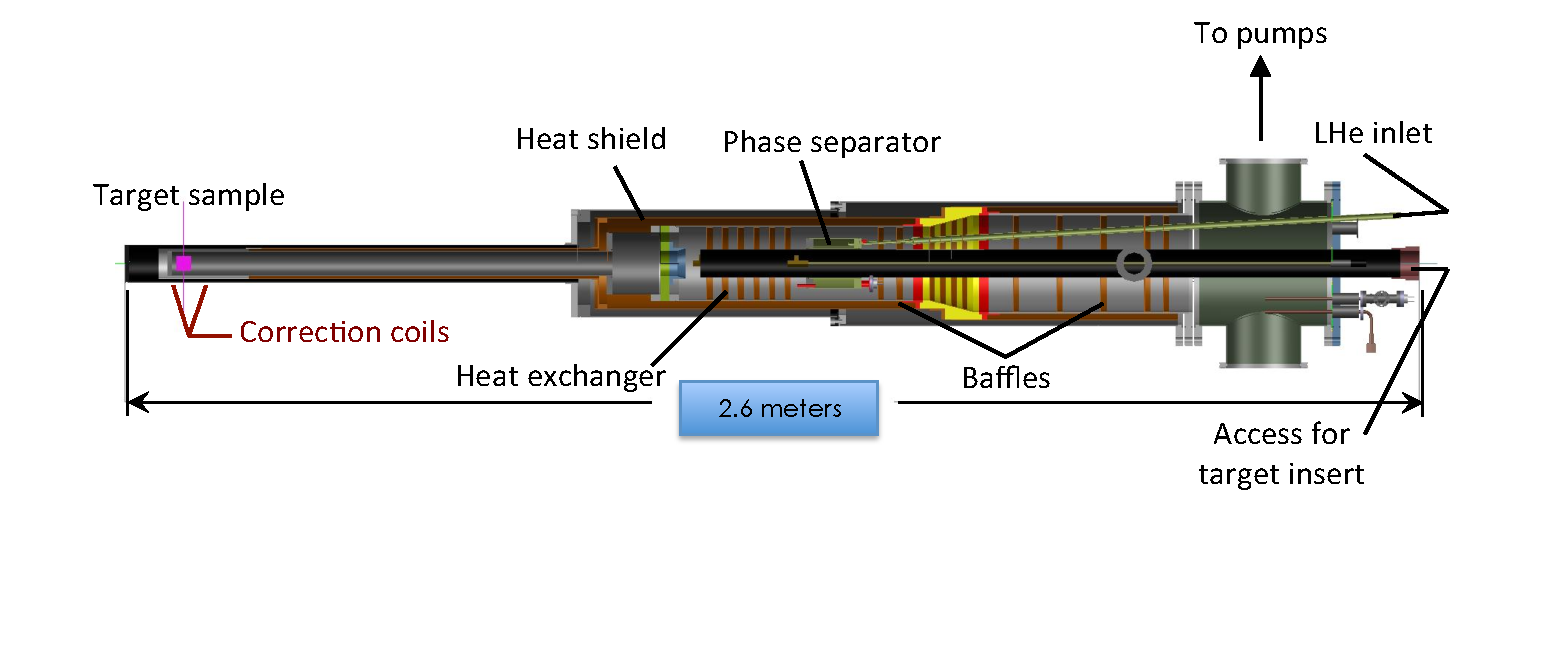
\includegraphics[width=5.5in]{Target_Side.pdf}
\end{center}
\caption{Side view of the CLAS12 dynamically polarized target.}
\label{Target}
\end{figure}
The proposed experiment will utilize a new, dynamically polarized target under construction for the CLAS12 spectrometer by a collaboration of the Jefferson Lab Target Group, the University of Virgina, Old Dominion University and Christopher Newport University.  The target cryostat, shown schematically in Figure~\ref{Target}, is specifically designed according to the geometrical constraints imposed by the CLAS12 detector package, primarily the Silicon Vertex Tracker.  Frozen, deuterated ammonia has been chosen as the target material for its high deuteron content (30\% by weight), high deuteron polarization (up to 50\%), and high resistance to radiation damage \cite{Goertz2002}.  Construction of the target is currently underway, with initial tests anticipated in 2017.

To realize Dynamic Nuclear Polarization (DNP), a dielectric solid is doped with a small concentration 
($10^{19}$~cm$^{\minus3}$) of paramagnetic radicals.  The unpaired electrons in the radicals are highly polarized by cooling the sample to a low temperature and applying a strong magnetic field.  For example, at the proposed operating conditions of 1~K and 5~T, the electron polarization is greater than 99.99\%.  Off-center microwave saturation of the electron spin resonance drives mutual electron/nuclear spin flips which effectively transfer the electron polarization to the nuclei.  Either positive or negative nuclear polarization can be realized, depending on whether the microwave frequency is slightly below or above the electron resonance frequency of 140~GHz.

The target sample will be cooled to 1~K by a bespoke $^4$He evaporation refrigerator with an anticipated cooling power of about 0.5~W at 1.0~K.  The CLAS12 solenoid shall provide the necessary 5~T magnetic field.  For optimum polarization, the uniformity of the field should be about 100 ppm or better over the volume of the sample.  If the solenoid is unable to provide this level of uniformity, it may be necessary to include small superconducting correction
coils inside the target cryostat, or to reduce the sample dimensions.  

\subsubsection{Luminosity}\label{sec_luminosity}
The nominal length of the target container will be $L=4.0$~cm, with a 2.5~cm diameter. 
It will be filled with mm-sized granules of frozen $^{14}$ND$_3$ with a density $\rho =$ 1.007 g/cm$^3$ and a packing fraction $f\approx0.6$.  The total luminosity with electron beam intensity $I$ will be 
\begin{eqnarray}
	\mathcal{L}  & = & f \rho L N_A I   \\
& = & 0.6(1.007\, {\rm g/cm}^3)(4.0\,{\rm cm})(6.02\times10^{23}\,{\rm g}^{\minus 1})(6.24\times10^9\,{\rm s}^{-1}{\rm nA}^{\minus 1}) \nonumber \\
	                   & = & 9.1 \times 10^{33} \, {\rm cm}^{\minus 2} \,{\rm s}^{\minus 1} \,{\rm nA}^{\minus 1} \nonumber
\end{eqnarray}
Note that this number is per nA of incident beam current.  
The luminosity for scattering from polarized neutrons
within the deuterons will be $3/20$ of the above number, or 
$1.4 \times 10^{33}\,{\rm cm}^{\minus 2} \, {\rm s}^{\minus 1} \, {\rm nA}^{\minus 1}$.
We anticipate running most of the experiment at 10~nA, giving a neutron luminosity of $1.4\times10^{34} 
\,{\rm cm}^{\minus 2} \, {\rm s}^{\minus 1}$.  An additional 10 days using the Forward Tagger will be run at a reduced beam current of 5~nA.  In order to reduce effects due to localized beam heating and radiation damage, the beam will be continuously rastered over 2.4~cm of the 2.5~cm target diameter.


\subsubsection{Polarization measurement}\label{sec_target_polarization}
The deuteron polarization will be monitored online by continuous wave NMR, using the industry standard
Liverpool Q-meter \cite{Court1993}.    There are two means whereby the polarization can be extracted from the NMR signal: the area method and the peak-height method.  We intend to use both, and either should provide a relative uncertainty $\Delta P/P \approx 4$\%.  We also intend to extract the polarization offline using the
quasi-elastic scattering asymmetry.

First, the total area of the NMR absorption signal is proportional to the vector polarization of the sample, and the constant of proportionality can be calibrated against the polarization of the sample measured under thermal equilibrium (TE) conditions.  This is the standard method used for polarized proton targets, but can be more problematic for deuteron targets.  Typical conditions for the TE measurements are 5~T and 1.4~K,
where the deuteron polarization is only 0.075\%, compared to 0.36\% for protons.
This smaller polarization, along with quadrupolar broadening, makes the deuteron TE signal more difficult to measure with high accuracy.
We therefore intend to implement a straightforward modification to the NMR circuit that has been shown to improve the stability and signal-to-noise ratio of the NMR signal~\cite{Court2004}. This modification was 
successfully utilized during the eg1-DVCS experiment in Hall B.  

Second, the deuteron polarization can also be extracted from the {\em shape\/} of the NMR signal.  
The deuteron is a spin-1 nucleus with three magnetic substates, $m=\minus1, 0, \plus1$, and the 
NMR absorption signal is a superposition of the $\minus 1-0$ and $\plus 1-0$ transitions.
In the case of ${}^{14}$ND$_3$, the deuteron's electric quadrupole moment interacts with electric field gradients within the molecule and splits the degeneracy of the two transitions.  The degree of splitting depends on the 
angle between the magnetic field and direction of the electric field gradient.  The resultant line shape, integrated over a sample of many polycrystalline beads, has the form of a Pake doublet (see Fig.\/\ref{NMR}).  
It has been experimentally demonstrated that, at or near steady-state conditions, the magnetic substates of deuterons in dynamically polarized ${}^{14}$ND$_3$ are populated according to the Boltzmann distribution with a characteristic {\em spin\/} temperature $T_s$ that can be either positive or negative, depending on the sign of the polarization. In this case, the vector polarization can be determined by the
ratio of the two transition intensities, $r=I_{\plus} / I_{\minus}$ \cite{Dulya1997}:
\begin{equation}
P_z = \frac{(r^2-1)}{(r^2 + r +1)}.
\end{equation}
An online estimate of the polarization can be made by comparing the heights of the two peaks.  
For a more accurate determination, an offline analysis of the entire line shape is necessary \cite{Dulya1997}.

\begin{figure}
\begin{center}
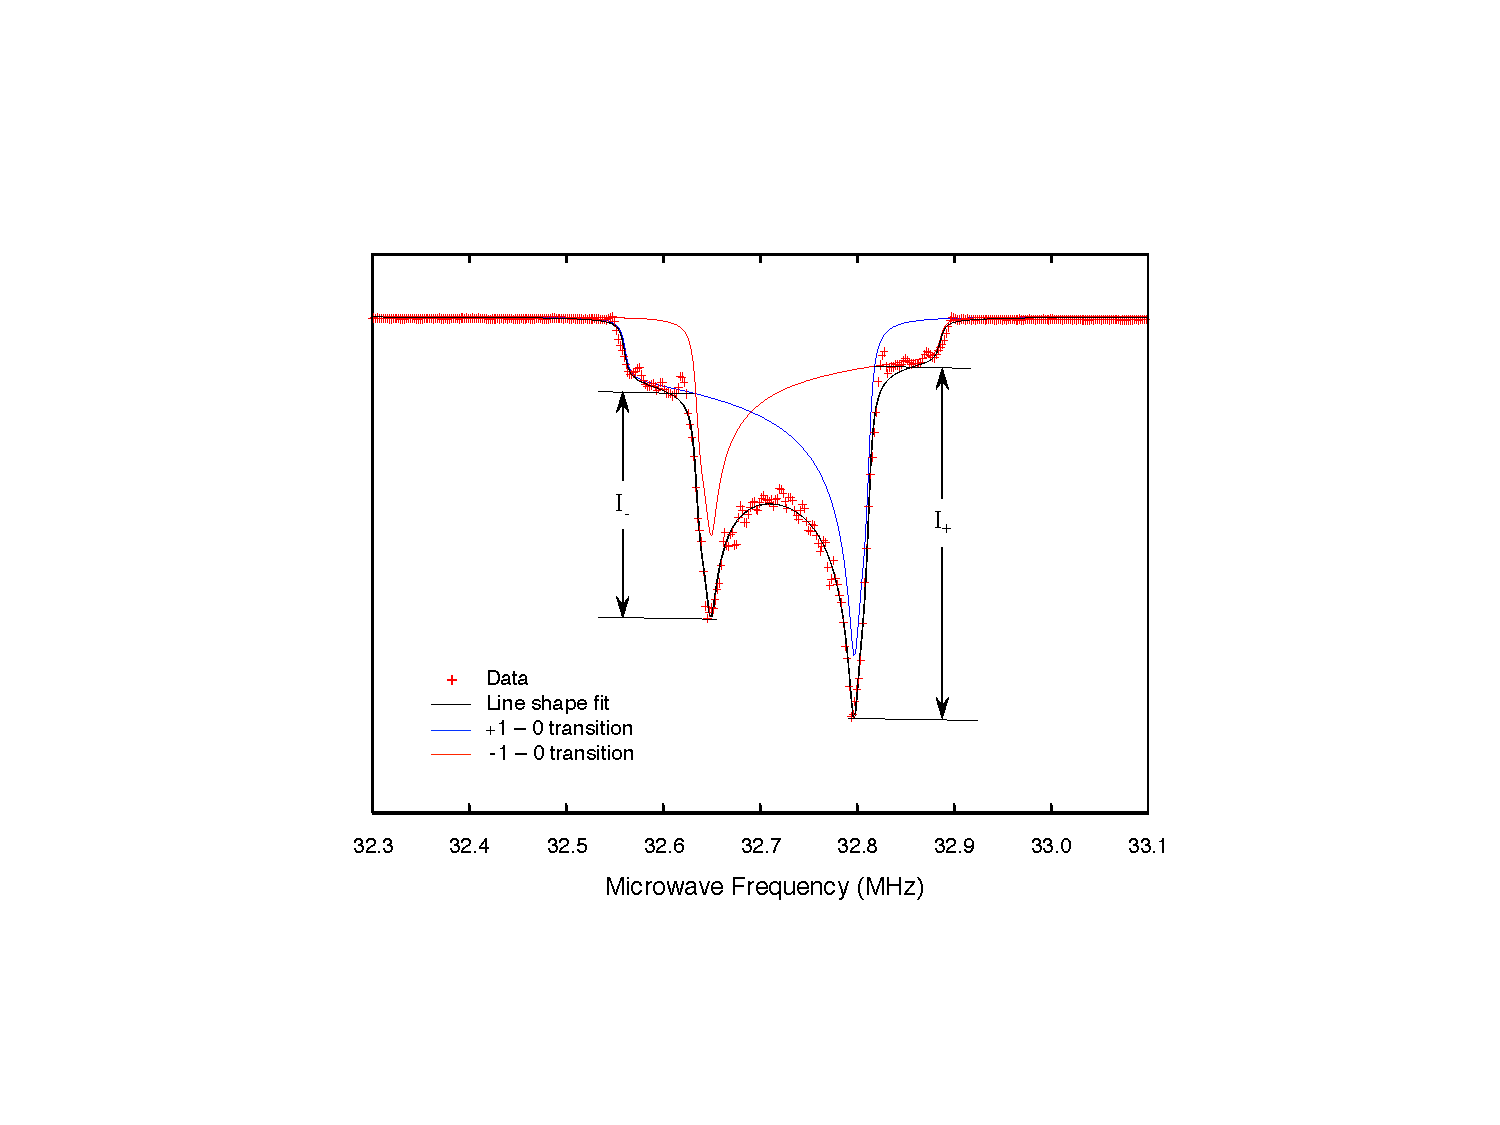
\includegraphics[width=3in]{Stache_NMR.pdf}
\end{center}
\caption[Typical ${}^{14}$ND$_3$ NMR signal]
{Typical NMR signal of polarized ${}^{14}$ND$_3$.  The black line results from a sophisticated line shape 
analysis of the data points and is a superposition of the two NMR transitions shown in red and blue.
This figure is adapted from~\cite{Kwaltine2013}.}
\label{NMR}
\end{figure}

Finally, the polarization will also be studied offline using the experimental data. We will extract the product of the beam and target polarization, $P_b P_t$, by measuring the quasi-elastic asymmetry ($\vec{d}(e,e'p)$) and by comparing it with the known theoretical value:
\begin{equation}
  P_b P_t=\frac{1}{D_f}\frac{A_{meas}}{A_{theo}}
\end{equation}
where $D_f$ is the dilution factor to account for the contribution of the unpolarized background (Section~\ref{sec_dilution}).
The target polarization value, needed for the TSA, will be then computed by taking the ratio of $P_bP_t$ and  the value of the beam polarization $P_t$, measured in dedicated M{\o}ller polarimetry runs. 

\subsubsection{Overhead for target operation}\label{sec_target_over}
There are four routine target operations that must be considered as overhead. 
First, we intend to provide an initial dose of approximately 20~Pe$^{\minus}$/cm$^2$ at 200~nA to each target sample prior to its use in the nDVCS experiment.\footnote{1 Pe$^{\minus} = 10^{15}$ electrons.}  This is necessary to achieve the highest possible deuteron polarization, as is explained below.  Second, the target must be periodically warmed to approximately 100~K in order to repair the deleterious effects of radiation damage, a process known as annealing.  Third, the target sample must be replaced when the anneals become ineffective at repairing the radiation damage.  Fourth, the NMR system will be periodically calibrated by performing
measurements of the thermal equilibrium polarization of deuterons at 5~T and temperatures around 1.4~K.
We examine each of these in the following sections, and a summary is made at the end.
Note that most overhead operations do not require the CEBAF electron beam, and are 
therefore counted as calendar days, not PAC days (one calendar day = two PAC days).
The only exception is the initial cold dose of electrons, as described below. Please note that this overhead estimate is for the total 110 days of beam time, consisting of 50 already-approved days and the additional 60 requested in this proposal. The target overhead is about the same for each. 

\vspace{-.15in}
\paragraph{Cold dose:}
In solid ammonia, paramagnetic radicals are created within the target sample by ionizing radiation, usually 
in the form of a 10--20~MeV electron beam, at a dose of about 
100~Pe$^{\minus}$/cm$^2$.
This is usually applied with the material cooled to 90~K with liquid argon, after which it may be stored indefinitely in liquid nitrogen.  
In the case of {\em deuterated\/} ammonia, experience has shown that polarizations greater than 20\% are only achieved after an additional  ``cold'' dose of approximately 10~Pe$^{\minus}$/cm$^2$ 
has been applied to the sample at 1~K.  
During the EG4 program in Hall B, the deuteron polarization increased from an initial value under 20\% to more than 45\%  after a cold dose of  20~Pe$^{\minus}$/cm$^2$~\cite{Slifer2007}.  In this case, the CLAS detectors were turned off and a 100~nA beam was applied to the sample for an hour or so, followed by a 100~K anneal.  These cold irradiations were interspersed with normal data-taking at 2~nA, and the deuteron polarization was observed to increase after each anneal, eventually exceeding 45\%.  Rather than following this prescription, we intend to prepare each target sample with a 20~Pe$^{\minus}$/cm$^2$ cold dose before using it in the experiment.  The CLAS12 detectors will be turned off for this procedure, which will require about a day for each sample at 200~nA. 

\vspace{-.15in}
\paragraph{Annealing:}
As a solid polarized target material, deuterated ammonia has a remarkably high resistance to radiation damage, 
exceeded only by lithium hydride and lithium deuteride.
When exposed to ionizing radiation, the decay of the polarization is roughly exponential in manner,
\begin{equation}
  P = P_o e^{-D/\delta}.
\end{equation}
Here $D$ is the dose, measured in Pe$^{\minus}$/cm$^2$.
The critical dose $\delta$ of ND$_3$ is different for the positive and negative spin states, with
$\delta_{\plus} = 13$~Pe$^{\minus}$/cm$^2$ and
$\delta_{\minus} = 26$~Pe$^{\minus}$/cm$^2$~\cite{Goertz2002}.
The polarization decay is due to the creation of additional paramagnetic species
that do not contribute directly to the DNP process, but do contribute to the spin-lattice 
relaxation of the nuclear spins.
Fortunately, the concentration of these new radicals can be reduced by annealing the target sample at temperatures up to about 100~K for some tens of minutes.

For the purposes of this proposal, we assume an initial polarization of 45\%, 
which has been achieved in both the Hall C polarized target and the original Hall B
polarized target.  To maintain an average polarization of 40\%, the radiation 
damage must be repaired by annealing the target sample when the polarization 
falls to 35\%, or in other words, when the dose reaches 
$\minus \ln(\frac{0.35}{0.45})\delta \approx 5$~Pe$^{\minus}$/cm$^2$.  
Here we have used the average value of $\delta_{\plus}$ and $\delta_{\minus}$.  
Assuming a 10~nA beam current distributed evenly over a 2.4~cm diameter, 
this dose will be accumulated, on average, after 4 days.  We estimate a total of four
hours will be required to anneal the target, cool it back to 1~K, and repolarize it to 40--45\%.

\vspace{-.15in}
\paragraph{Target lifetime:}
During 100 days of beam time at 10~nA, the polarized target
will accumulate a total dose of 120~Pe$^-$/cm$^2$, while an additional 10 days at 5~nA will deposit
6~Pe$^-$/cm$^2$.
However, the maximum that a ND$3$ sample can tolerate before it must be replaced is not fully known.  
McKee~\cite{McKee2004} reports that for the Gen01 experiment in Hall C, a total of dose of
315~Pe$^{\minus}$/cm$^2$ was deposited on six different samples, and at least one continued to give high polarizations even after a dose of 100~Pe$^{\minus}$/cm$^2$.  The total dose had little or no effect on the frequency of anneals, although the maximum attainable polarization did decline slightly after about 
50~Pe$^{\minus}$/cm$^2$.   For this proposal we make the conservative estimate that the samples will be replaced after a total dose of 50~Pe$^{\minus}$/cm$^2$, of which 20~Pe$^{\minus}$/cm$^2$
will occur before data-taking begins.  The remainder will be incurred after about
25~days of data-taking at 10~nA, and so we anticipate that four samples of ND$_3$ will be sufficient 
for the entire experiment, with one sample incurring an additional 6~Pe$^-$/cm$^2$ 
for the Forward Tagger runs.  Dedicated carbon runs will occur between the ND$_3$ sample changes.
The time required to replace an old ND$_3$ sample with the carbon target, then replace the carbon with fresh
ND$_3$, perform a TE calibration on the new sample and polarize it to 40--45\% should be about 12 hours. Note that this does not include the actual time spent acquiring data on the carbon target.

\vspace{-.15in}
\paragraph{TE measurements:}
Thermal equilibrium (TE) measurements are necessary to calibrate the NMR system,
and must be performed whenever a new target sample is introduced into the experiment.  Additional
measurements are made throughout the experiment in order to monitor and reduce sources of systematic uncertainty such as gain drift and settling of the sample beads.   
To perform a TE, the target sample must first have its existing dynamic polarization destroyed, either by temporarily warming the sample or temporarily lowering the magnetic field to zero.  The sample must then be allowed to achieve its thermal equilibrium polarization, which it approaches in an exponential manner with a spin-lattice time constant $T_1$ that depends on the field strength, the sample's temperature, and its density of paramagnetic radicals. Since annealing the sample reduces its radical density and increases $T_1$, 
it is best to do TEs prior to the anneals.  Most measurements are made around 1.4~K, where the signal size is not too small, and $T_1$ is not too long.
Because the deuteron TE signal is small, a significant amount of signal averaging must be utilized to achieve a precise determination of its area, and so the time required for each measurement will depend strongly on the signal-to-noise ratio of NMR system.  Based on past experience, we assume six hours will be sufficient.  This includes the time required to polarize the sample to 40-45\% at the end of the calibration.

\vspace{-.15in}
\paragraph{Target overhead summary:}
Based on the above information we provide the following estimate for the total overhead necessary to operate the polarized target.  The total is about 8 PAC days.  Whenever possible, anneals, TE measurements, and target changes can be coordinated with scheduled or unscheduled beam outages to lessen their impact on data acquisition and further reduce the overhead.  
%One possible sequence is indicated in Fig.~\ref{Operation}.
%\begin{figure}[ht]
%\begin{center}
%includegraphics[width=5.in]{Operation.pdf}
%\end{center}
%\caption[Possible target operation sequence]
%{One possible sequence of target operations for the 80 day experiment. The numbers indicate the total dose accumulated during data taking, in Pe$^-$/cm$^2$. The experiment ends after 95~Pe$^-$/cm$^2$.
%{\bf CD}: Cold Dose.  {\bf TE}: Thermal Equilibrium measurement.  {\bf A}: Anneal. }
%\label{Operation}
%\end{figure}
\begin{enumerate}
  \item{Cold dose of 20~Pe$^{\minus}$/cm$^2$ at 200~nA.  Required: 4 @ 24 hours each. 
    Total: 96 PAC hours.}  
    \item{Anneal every 5~Pe$^{\minus}$/cm$^2$.  Required: 22 @ 4 hours each. 
      Total: 88 calendar hours = 44 PAC hours.}
      \item{Change target sample after 30~Pe$^{\minus}$/cm$^2$.  Required: 3 @ 12 hours each.  
      Total: 36 calendar hours = 18 PAC hours.}
        \item{TE calibration of NMR system at the beginning of each target sample, and after 
          15~Pe$^{\minus}$/cm$^2$.  Required: 12 @ 6 hours each.  
          Total: 72 calendar hours = 36 PAC hours}.
\end{enumerate}

\begin{figure}
\begin{center}
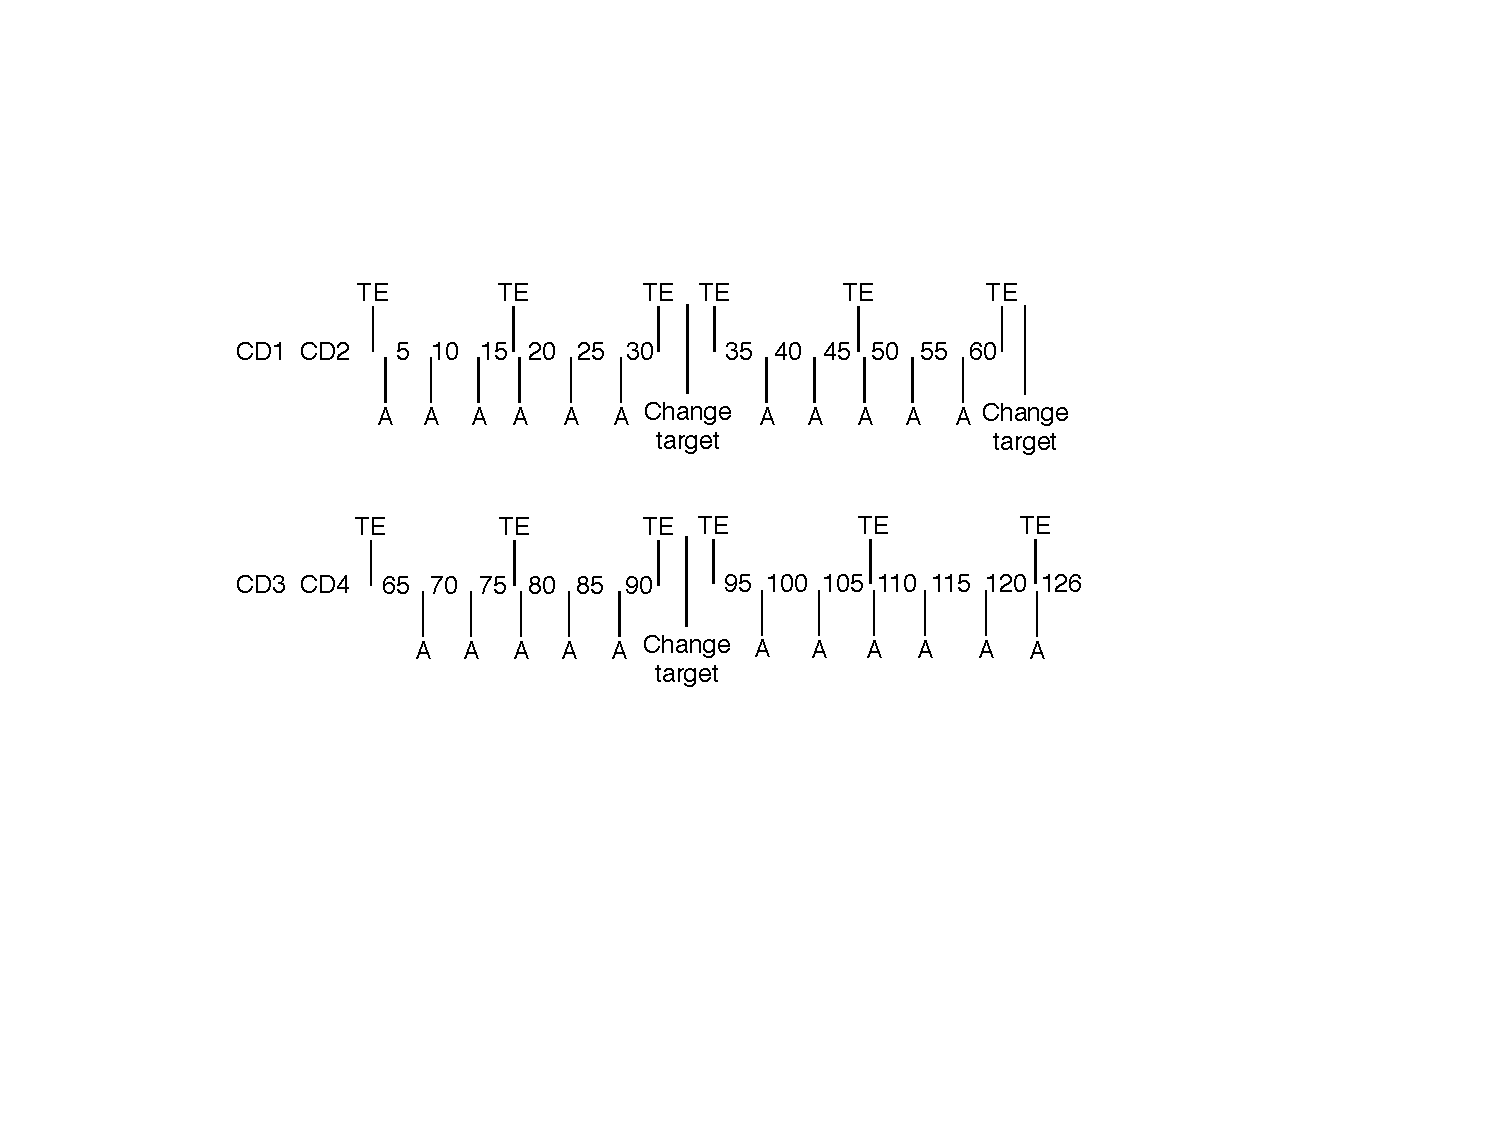
\includegraphics[width=6in]{Operation_110days.pdf}
\end{center}
\caption[Overhead operations of the target]
{One possible sequence of target operations for the entire 110-day experiment. The top half represents the 50 days of already-approved beam time, and the bottom half the 60 days of extension. The numbers indicate the total dose accumulated during data taking, in Pe$^-$/cm$^2$. The experiment ends after 126 Pe$^-$/cm$^2$. 
{\bf CD:} Cold Dose. {\bf TE:} Thermal Equilibrium measurement. {\bf A:} Anneal.}
\label{Operation}
\end{figure}

